%!xelatex = 'xelatex --halt-on-error %O %S'

\documentclass{thuemp}
\usepackage{lipsum}  % 生产假书乱文的包,实际使用时可去掉
\begin{document}

% 标题,作者
\emptitle{PID 控制在医学麻醉过程血压控制中的应用}
\empauthor{秦华谦}{李中华老师}

% 奇数页页眉 % 请在这里写出第一作者以及论文题目
\fancyhead[CO]{{\footnotesize 秦华谦: PID 控制在医学麻醉过程血压控制中的应用}}


%%%%%%%%%%%%%%%%%%%%%%%%%%%%%%%%%%%%%%%%%%%%%%%%%%%%%%%%%%%%%%%%
% 关键词 摘要 首页脚注
%%%%%%%%关键词
\Keyword{PID控制, 麻醉, 血压控制}
\twocolumn[
\begin{@twocolumnfalse}
\maketitle

%%%%%%%%摘要
\begin{empAbstract}
本文基于PID控制系统开发了一个系统,旨在自动测量和控制多种生命参数,以保持其在适当范围内。其目标是提高手术中麻醉师的安全性。为了进一步优化系统性能,我们进行了一项专门的研究,通过对kp、ki、kd三个参数的调整,探究PID系统内不同参数对系统响应的影响。该系统实现了自动调节麻醉深度,以减小波动和冲击响应。实验结果表明,引入设计的控制器后,血压控制系统对于给定输入信号的超调量减小,调节时间缩短。在阶跃输入信号下的稳态误差为零,并在阶跃扰动输入信号下能保持稳态误差在一定范围内,最终实现稳态输出为零。
\end{empAbstract}

%%%%%%%%英文标题、作者、摘要、关键词
\emptitleEn{Application of PID control in blood pressure control in medical anesthesia process}
\empauthorEn{Huaqian Chin}{Prof. Li Zhonghua}
\KeywordEn{PID control, anaesthetization, blood pressure control}

\begin{empAbstractEn}
This article has developed a system based on the PID control system, aimed at automatically measuring and controlling various vital parameters to maintain them within an appropriate range. The goal is to enhance the safety of anesthesiologists during surgery. To further optimize system performance, we conducted a dedicated study, investigating the impact of different parameters in the PID system on system response by adjusting the kp, ki, and kd parameters. The system achieves automatic adjustment of anesthetic depth to minimize fluctuations and impact responses. Experimental results show that after introducing the designed controller, the overshoot of the blood pressure control system for a given input signal decreases, and the adjustment time shortens. The steady-state error under step input signals is zero, and under step disturbance input signals, it can maintain the steady-state error within a certain range, ultimately achieving a steady-state output of zero.
\end{empAbstractEn}

%%%%%%%%首页角注,依次为实验时间、报告时间、学号、email
\empfirstfoot{2023-05-20}{2023-5-30}{21312683}{qinhq5@mail2.sysu.edu.cn}
\end{@twocolumnfalse}
]
%%%%%%%%!首页角注可能与正文重叠,请通过调整正文中第一页的\enlargethispage{-3.3cm}位置手动校准正文底部位置:
%%%%%%%%%%%%%%%%%%%%%%%%%%%%%%%%%%%%%%%%%%%%%%%%%%%%%%%%%%%%%%%%
%  正文由此开始
\wuhao 
%  分栏开始

\section{引~~言}
\enlargethispage{-3.3cm}
手术中麻醉师需监测多种生命参数,如:麻醉
深度、血压、心率、体温、血氧、呼气中二氧化碳
浓度等,并将它们控制在适当的范围内。能够自动
测量、控制某些生命参数,能够提高受术者的安
全。我们希望开发一个自动调节麻醉深度的系
统,病人的安全是最终目标。

许多麻醉师将平均动脉压作为麻醉深度最可
靠的度量。根据临床经验和麻醉师所遵从的程序,
被控变量确定为平均动脉压(MAP)。

本文主要是运用 PID 控制器的设计方法,对
麻醉过程中的血压控制模型进行控制器的设计,通过对kp、ki、kd三个参数的调整,探究PID系统内不同参数对系统响应的影响。
并且针对 PI,PD,PID 三种控制器在有无扰动两种情况下
进行性能分析的比较。

\section{实验原理}


\subsection{PID控制原理}

PID控制是一种常用的反馈控制算法,用于调节和稳定系统的输出。它的名称代表比例(Proportional)、积分(Integral)和微分(Derivative),分别表示控制器的三个主要组成部分。

比例控制(Proportional Control)是PID控制的基本部分之一。它通过将当前误差与一个比例常数相乘,产生一个控制量,用于调节系统输出。比例控制的作用是使系统对误差做出直接的响应,但它无法解决误差积累和系统超调等问题。

积分控制(Integral Control)是PID控制的第二个组成部分。它将误差的积分值与一个积分常数相乘,产生一个控制量。积分控制的作用是消除稳态误差,即系统输出与期望输出之间的差异。通过积分控制,系统可以逐渐减小并消除持续的误差。

微分控制(Derivative Control)是PID控制的最后一个组成部分。它通过将误差的变化率与一个微分常数相乘,产生一个控制量。微分控制的作用是抑制系统的超调和振荡,并提高系统的响应速度。通过微分控制,系统可以更快地调整输出,以适应误差变化的速率。

PID控制器将比例、积分和微分控制相结合,通过对误差的不同方面进行调节,实现对系统输出的精确控制。PID控制器的输出值由三个控制分量的加权和得出,即:

输出 = 比例控制 + 积分控制 + 微分控制

通过调整比例常数、积分常数和微分常数,可以对PID控制器进行参数调优,以满足不同系统的需求。调优过程通常包括实验、观察和调整,以获得最佳的控制效果。

总而言之,PID控制是一种基于反馈的控制算法,通过比例、积分和微分控制三个部分的相互作用,实现对系统输出的精确调节。它广泛应用于自动控制领域,用于稳定系统、消除误差和提高响应速度。

\subsection{系统设计流程图}
\begin{figure}[H]
\centering
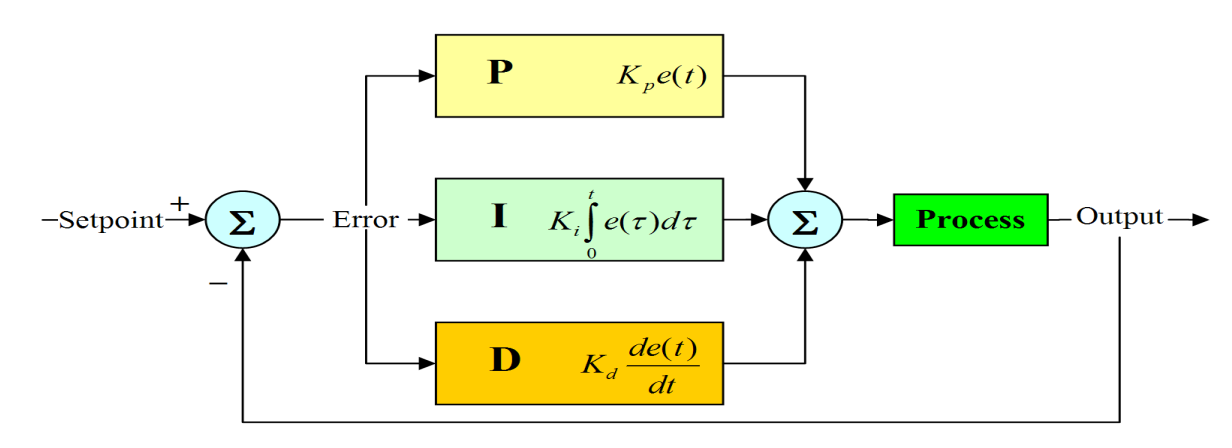
\includegraphics[width=0.8\linewidth]{./img/from_internet/PID.png}
\end{figure}

\subsection{系统参数介绍}

PID 控制器的比例单元 (P)、积分单元 (I) 和微分单元 (D) 分别对应目前误差、过去累计误差及未来误差。借由调整 PID 控制器的三个参数,可以调整控制系统,设法满足设
计需求。

PID控制器(比例-积分-微分控制器)的参数选择取决于具体的应用场景和系统的动态特性。通常,这些参数需要通过一些调参方法(例如Ziegler-Nichols方法)进行调整,以达到系统的稳定性和性能需求。

PID控制器的三个参数分别为:

1. P(比例):该参数控制系统的响应速度。P参数越大,系统对错误的反应越快,但如果过大,可能会导致系统不稳定。

2. I(积分):该参数控制系统是否能达到设定点(或称为参考点)。I参数可以消除系统的静差,但如果过大,可能会导致系统超调和震荡。

3. D(微分):该参数控制系统的稳定性。D参数可以预测系统的行为,减小系统的超调,但如果过大,可能会引入噪声,使系统不稳定。

在实际应用中,PID参数的调整是一项复杂的工程任务,需要根据系统的具体特性和性能需求进行优化。有时,人们也使用一些自适应的PID控制算法,如模糊PID,遗传算法等,以自动地优化PID参数。


\section{实验过程}

\subsection{系统设计流程图}
\begin{figure}[H]
\centering
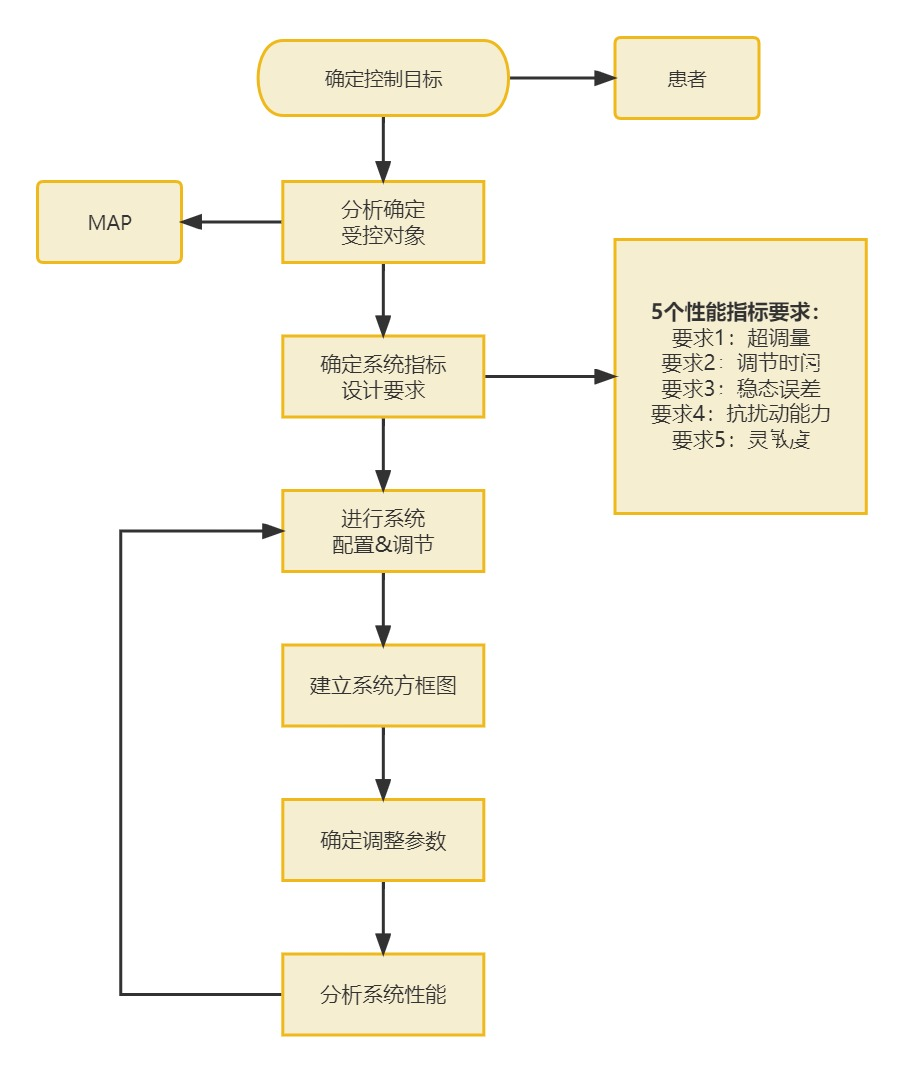
\includegraphics[width=0.8\linewidth]{./img/work_stream.jpg}
\end{figure}


\subsection{控制目标与实验要求}

麻醉过程中的血压控制系统控制目标:
\begin{itemize}
	\item 控制对象: 需麻醉的患者
	\item 控制任务: 将患者 MAP 调节到任意预期设定的水平,并在存在干扰信号的情况下将 MAP维持在预期设定的水平。
	\item 受控变量: MAP(平均动脉压)
	\item 系统输入:MAP的期望值
	\item 干扰输入: 手术干扰,噪声干扰
	\item 误差量: 稳态误差 = 输入 - 输出
	\item 系统输出: 实际的 MAP 量
\end{itemize}

该控制系统的实验设计要求:
\begin{enumerate}
	\item 取N(s)=0, Td(s)=0
	
  \begin{itemize}
    \item 基于PD、 PI控制器对系统进行Matlab仿真。
    
    \begin{itemize}
      \item 在PD或PI控制器中,固定一个参数,调节另外一个参数,观察输出结果的变化
    \end{itemize}

    \item 基于PID控制器对系统进行Matlab仿真
    \begin{itemize}
      \item 改变三个参数的值,看在不同的组合下,观察系统的输出的变化
    \end{itemize}
    
  \end{itemize}

	\item 取N(s)=0, Td(s)=50/s
	\begin{itemize}
    \item 重复上面的仿真过程
  \end{itemize}
  
\end{enumerate}



\subsection{系统设计}

其中, $R(s)$和$Y (s)$分别为期望的平均动脉压变化和实际的平均动脉压变化, 
两者的偏差被控制器用于确定对泵的阀门给定值,泵/蒸发器给患者输送麻醉蒸汽。
而$𝑇𝑑(s)$和$𝑁(s)$分别为手术过程中的扰动和噪声, $G_c (s)$为待加入的控制器传递函数。
另外, G(s)是被控对象, 其传递函数为
\begin{equation}
G(s)=1/(s+p)^2\
\end{equation}

传感器H(s)传递函数为
$$ H\left(s\right)=1 $$

泵的传递函数为$G_p(s)$,为
$$ G_{p\left(s\right)}=\frac{U(s)}{V(s)}=\frac{1}{s} $$

\subsection{传递函数设计与解析}

通过对信号方框图的分析,我将R & Td & N 分别作为输入,重绘信号方框图

\begin{figure}[H]
\centering
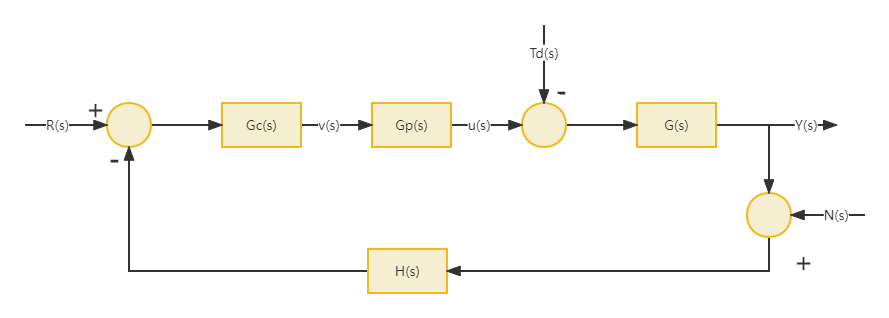
\includegraphics[width=0.8\linewidth]{./img/Rs.png}
\caption{$Rs(s)$作为输入} 
\end{figure}

\begin{figure}[H]
\centering
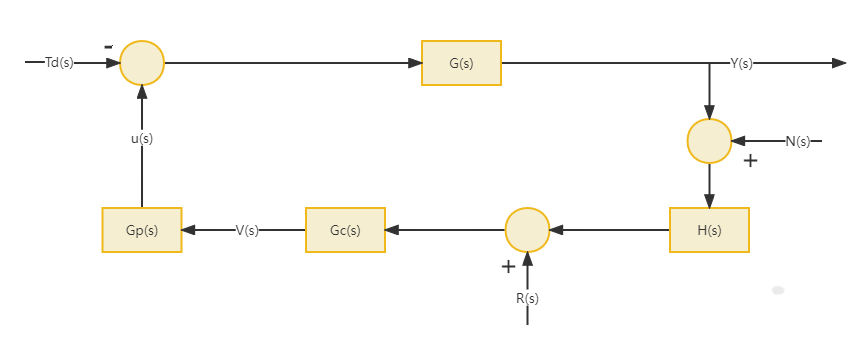
\includegraphics[width=0.8\linewidth]{./img/Td.png}
\caption{$Td(s)$作为输入} 
\end{figure}

\begin{figure}[H]
\centering
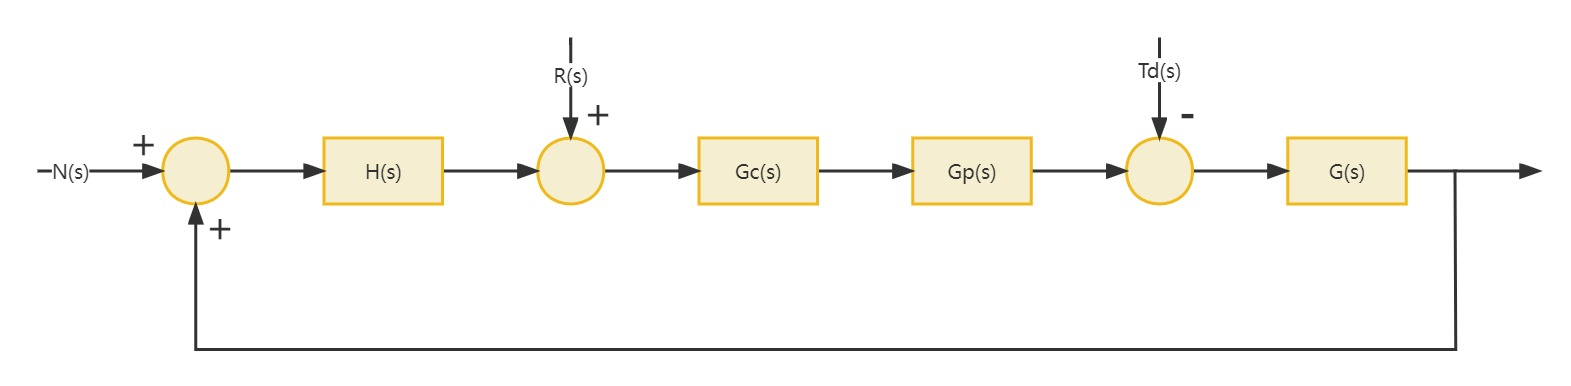
\includegraphics[width=0.8\linewidth]{./img/N.jpg}
\caption{$N(s)$作为输入} 
\end{figure}

根据三幅信号框图,写出闭环传递函数如下:

以$R(s)$作为输入
$$
\emptyset_r(s)=\frac{G_c(s)\ast G_p(s)\ast G(s)}{1+H(s)\ast G_c(s)\ast G_p(s)\ast G(s)}
$$
以$R(s)$作为输入
$$
\emptyset_{Td}\left(s\right)=\frac{G(s)}{1+H\left(s\right)\ast G_c\left(s\right)\ast G_p\left(s\right)\ast G\left(s\right)}
$$
以$R(s)$作为输入
$$
\emptyset_n(s)=\frac{H(s)\ast G_c(s)\ast G_p(s)\ast G(s)}{1+H(s)\ast G_c(s)\ast G_p(s)\ast G(s)}
$$

\subsection{PID系统传递函数}
$$
G_c\left(s\right)=\frac{K_ds^2+K_ps+K_i}{s}
$$
% ========================================================================================
% ========================================================================================


\subsection{二级标题}
正文内容正文文字五号宋体正文内容正文文字五号宋体正文内容正文文字五号宋体正文内容正文文字五号宋体正文内容正文文字五号宋体正文内容正文文字五号宋体正文内容正文文字五号宋体正文内容。

\section{实验结果与分析}
一般先给出实验条件、现象和实验结果,然后用学过的物理理论结合实验条件做出合理的分析和解释。

实验数据及处理结果在报告中以图或表形式给出,并对图、表所反映的现象或物理规律做出具体说明和解释。图、表格式规范,大小适中。

分析讨论影响实验结果的因素,改进方法等

\subsection{往届学生报告中常见问题与不足}
正文内容正文文字五号宋体正文内容正文文字五号宋体正文内容正文文字五号宋体正文内容正文文字五号宋体正文内容正文文字五号宋体正文内容正文文字五号宋体正文内容。
\subsubsection{三级标题}
\subsubsection{只给数据和结果,没有对结果所反映的物理规律做理论分析及数据误差分析;}
\subsubsection{数据及结果直接给出,没有必要的实验条件说明和所用物理计算公式;}
\subsubsection{结果以图、表给出时,图、表不规范(缺少坐标分度、物理量及其单位等);}
正文内容正文文字五号宋体正文内容正文文字五号宋体正文内容正文文字五号宋体正文内容正文文字五号宋体正文内容正文文字五号宋体正文内容正文文字五号宋体正文内容。
\subsection{报告中公式、字母的规范写法}
公式全文统一编号,如公式为
\begin{equation}\label{EQ1}
\frac{\partial u}{\partial x}+\frac{\partial v}{\partial y}+\frac{\partial w}{\partial z}=0
\end{equation}
式中,$u$是××××(单位);$v$是×××(单位);$w$是××(单位)。

对于公式,应全文统一连续编号,如式\eqref{EQ1}……一般情况下,需要引用的或重要的公式才编号。在文中引用时,用“式(编号)”表示。
后文不再提及的,可以不编号。如
\begin{equation*}
1 + 1 + 3 = 5
\end{equation*}

对于公式中首次出现的量的符号,按照其在式中出现的顺序,用准确、简洁的语句对其进行逐一解释。公式中变量应尽量避免复合上下角标的使用;尽量少用3层关系的上下标,同时应尽量减少不必要的公式推导。

\subsection{报告中图的规范要求}
插图全文顺序编号。插图内容应与正文内容密切结合,每幅图前都应有相应的引出或介绍文字。图形应保证线条清晰,图形大小应适应版面要求,合理布局,图内如有标注或说明性文字时应清晰可辨。图中除了物理量符号及单位外一律用中文,同一图中的不同曲线应用不同线型表示。插图分辨率要大于600PPI。

正文文字中先见文,后见图,图号全文统一按顺序编号,如图\ref{fig:eg}所示。图中文字为6号,图线必须清晰可辨坐标轴的物理量和单位不可缺。


% \begin{figure}[H]
% \centering
% 
\includegraphics[width=0.8\linewidth]{./image/example.jpg}
% \caption{图片示例} \label{fig:eg}
% \end{figure}


\subsection{报告中表的规范}
推荐使用标准“三线表”(如表\ref{tab:eg1}所示。),内容易混淆时可加辅助线进行辅助说明。按表格在文中出现的顺序,用阿拉伯数字对其进行编号,全文顺序编号。应有相应的表题且每个表格前都应有相应的引出或介绍文字。

图、表应在文中有相应表述,即图、表的号应在文中引出,以先见文后见图、表为原则。每个图、表都必须有图名、表名,并且有编号。图号、表号应全文统一连续排列,即,应按照图1、图2……排列不应按小结编号。图片中的文字、线条应当清晰可辨,图片像素(DPI)在300以上。
表格推荐采用全线表,表头中使用量符号/量单位形式。如表\ref{tab:eg2}所示。

\begin{table}[h]
\centering
\captionnamefont{\wuhao\bf\heiti}
\captiontitlefont{\wuhao\bf\heiti}
\caption{三线表示例} \label{tab:eg1}
\liuhao
\begin{tabular}{cccc}
\toprule
{编号} &  {直径}/\si{\metre} & {静温}/\si{\kelvin} & {时间}/min\\
\midrule 
4 & 0.0349 & 268.15 & 30\\
5 & 0.01905 & 268.15 & 30\\
\bottomrule
\end{tabular}
\end{table}

\begin{table}[h]
\centering
\captionnamefont{\wuhao\bf\heiti}
\captiontitlefont{\wuhao\bf\heiti}
\caption{全线表示例} \label{tab:eg2}
\liuhao
\begin{tabular}{|c|c|c|c|c|}
\hline
U/V & I/mA & v/km·h$^{-1}$ & x/mm & p/MPa \\ \hline
\textit{12} & \textit{30} & \textit{80} & \textit{55} & \textit{110} \\ \hline
\textit{24} & \textit{34} & \textit{90} & \textit{60} & \textit{111} \\ \hline
\end{tabular}
\end{table}

\subsection{报告中英文缩略语的规范}
文中的英文缩略语应在首次出现时给出中文含义以及英文全称后再使用。例如,全球定位系统(Global Positioning System,GPS)。


\subsection{外文字母}
\subsubsection{斜体外文字母用于表示量的符号,主要用于下列场合}

\begin{enumerate}
\renewcommand{\labelenumi}{(\theenumi)}
\item 变量符号、变动附标及函数。
\item 用字母表示的数及代表点、线、面、体和图形的字母。
\item 特征数符号,如Re (雷诺数)、Fo (傅里叶数)、Al (阿尔芬数)等。
\item 在特定场合中视为常数的参数。
\end{enumerate} 

\subsubsection{正体外文字母用于表示名称及与其有关的代号,主要用于下列场合}
\begin{enumerate}
\renewcommand{\labelenumi}{(\theenumi)}
\item 有定义的已知函数(例如$\sin$, $\exp$, $\ln$等)。
\item 其值不变的数学常数(例如$\mathrm{e} = 2.718 281 8\cdots)$及已定义的算子。
\item 法定计量单位、词头和量纲符号。
\item 数学符号。
\item 化学元素符号。
\item 机具、仪器、设备和产品等的型号、代号及材料牌号。
\item 硬度符号。
\item 不表示量的外文缩写字。
\item 表示序号的拉丁字母。
\item 量符号中为区别其他量而加的具有特定含义的非量符号下角标。
\end{enumerate} 

\section{结~~论}
用准确、精炼的语言归纳总结使用的方法以及研究结果。

说明研究的创新价值和应用价值,包括对科技工作者的研究的价值和对产业发展的价值。

可说明自己做本实验的总结、收获和体会,对实验中发现的问题提出自己的建议。


%%%%%%%%%%%%%%%%%%%%%%%%%%%%%%%%%%%%%%%%%%%%%%%%%%%%%%%%%%%%%%%%
%  参考文献
%%%%%%%%%%%%%%%%%%%%%%%%%%%%%%%%%%%%%%%%%%%%%%%%%%%%%%%%%%%%%%%%
%  参考文献按GB/T 7714-2015《文后参考文献著录规则》的要求著录. 
%  参考文献在正文中的引用方法:\cite{bib文件条目的第一行}

\renewcommand\refname{\heiti\wuhao\centerline{参考文献}\global\def\refname{参考文献}}
\vskip 12pt

\let\OLDthebibliography\thebibliography
\renewcommand\thebibliography[1]{
  \OLDthebibliography{#1}
  \setlength{\parskip}{0pt}
  \setlength{\itemsep}{0pt plus 0.3ex}
}

{
\renewcommand{\baselinestretch}{0.9}
\liuhao
\bibliographystyle{gbt7714-numerical}
\bibliography{./TempExample}
}


\end{document}

